\documentclass[11pt]{article}
\usepackage[latin1]{inputenc}
\usepackage{a4wide}
\usepackage{amsmath}
\usepackage{amsfonts}
\usepackage{amssymb}
\usepackage{graphicx}
\usepackage{enumerate}
\usepackage{epstopdf}
\usepackage{float}
\usepackage{hyperref}

\title{Natural Computing, Assignment 1}
\author{Pauline Lauron - sXXXXXXX \and Dennis Verheijden - s4455770 \and Joost Besseling - sXXXXXXX}
\begin{document}
	\maketitle
	
	\section{}
	Due to no eliteness, we can treat the best member as any other member in the pool.
	
	\begin{enumerate}[(a)]
		\item There are 100 individuals, with a mean of 76. That means that the total size of the roulette wheel will be 7600. The current best member has a fitness of 157, so it will occupy $\frac{157}{7600}$th of the roulette wheel. This means that it has roughly a $2\%$ chance of being selected. If we select 100 members, we expect to select the best member $\frac{157}{7600} * 100 \approx 2 $ times.
		
		\item The chance that we don't select the fittest member is $1 - \frac{157}{7600}$. So the chance that we never select it is $\left(1 - \frac{157}{7600}\right)^{100} \approx 0.124$.
	\end{enumerate}

	\section{}
	
	The fitness function is \[ f(x) = x^2. \]
	
	The members of the pool are $x=3, x=5, \text{and} x=7$. So the total fitness is $3^2 + 5^2 + 7^2 = 83$. The chance to select each individual is: 
	\begin{itemize}
		\item[$x=3:$] $9/83 \approx 0.108$,
		
		\item[$x=5:$] $25/83 \approx 0.301$,
		
		\item[$x=5:$] $49/83 \approx 0.590$.
		 
	\end{itemize}

	When using the alternative selection function 
	\[
		f_1(x) = x^2 + 8,
	\] 
	
	the total fitness is $83 + 24 = 107$ and
	we obtain the following results: 
	
		\begin{itemize}
		\item[$x=3:$] $17/107 \approx 0.159$,
		
		\item[$x=5:$] $33/107 \approx 0.308$,
		
		\item[$x=5:$] $57/107 \approx 0.533$.
		
	\end{itemize}

We can see that the second function yields a lower selection pressure. This is because the relative boost of 8 is much higher for the less fit individuals. It almost doubles the fitness of the $x=3$ individual, and only amounts to a $0.16$-th increase in fitness of the $x=7$ individual.

\section{}
\begin{enumerate}[(a)]
\item When running the algorithm with $n=100$ for 1500 iterations, we can observe the result found in figure \ref{fig:mc}. We can see that the Monte-Carlo search as specified in the assignment did not find the optimal solution.

\item Running the algorithm ten times, the algorithm finds the optimal solution 0 times.

\end{enumerate}

\begin{figure}[H]
\centering
\includegraphics[width=0.75\textwidth]{images/monte_carlo.eps}
\caption{Monte Carlo Search for the Counting Ones problem, ran 10 times.}
\label{fig:mc}
\end{figure}

\section{}
\begin{enumerate}[(a)]
\item When running the (1+1)-GA algorithm for the Counting Ones problem, we found the results from figure \ref{fig:ga}.
\item As we can observe from our results, the algorithm found the optimum 10 times out of 10 runs.
\item If we compare these results to those of the Monte-Carlo algorithm, we can easily see that the Genetic Algorithm is a significant improvement, as the Monte-Carlo algorithm did not find the optimum once and the GA algorithm every time.
\end{enumerate}

\begin{figure}[H]
\centering
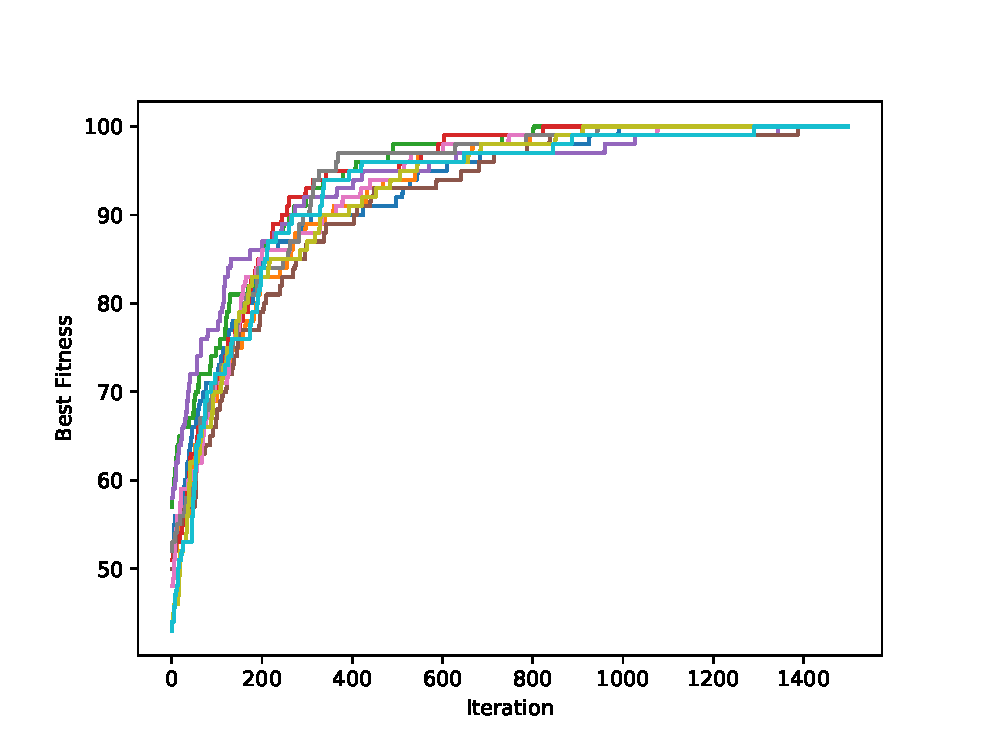
\includegraphics[width=0.75\textwidth]{images/ga.eps}
\caption{(1+1)-GA for the Counting Ones problem, ran 10 times.}
\label{fig:ga}
\end{figure}

\section{}
Suitable fonction : $F = \{\wedge,\rightarrow, \vee,\leftrightarrow \}$
\newline Terminal set : $T = \{x,y,z,true\}$
\newline S-expression : $ (\rightarrow (\land\ x\ true)(\lor (\lor\ x\ y)(\leftrightarrow z(\land\ x\ y))) $

\section{}
Something weird with symbolic expressions (programming)

\end{document}